\section{Séance 3 : Utilité et choix du consommateur}



\subsection{Courbes d'indifférence}
\begin{center}
	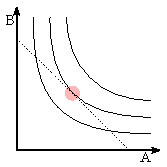
\includegraphics[width=0.25\textwidth]{images/graph_courbes_d_indifference.pdf}
\end{center}
$$TMS_{A,B}=\frac{UM_B}{UM_A}=-\frac{dA}{dB}$$
$$max(TMS_{A,B})=\frac{P_B}{P_A}$$
Contrainte budgétaire (pointié):
$$Budget=Y=P_A.A+P_B.B$$



\subsection{Cas particulier pour le budget}
si
$$U=k.X^A.Z^B$$
alors
$$Budget\ pour\ le\ bien\ X = \frac{A}{A+B}$$
$$Budget\ pour\ le\ bien\ Z = \frac{B}{A+B}$$



\subsection{Biens parfaitement complémentaires ou substituables}
\begin{center}
	\begin{tabular}{cc}
		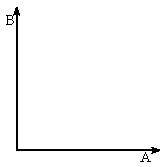
\includegraphics[width=0.25\textwidth]{images/graph_biens_parfaitement_complementaires.pdf}&
		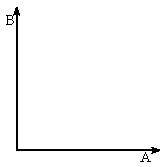
\includegraphics[width=0.25\textwidth]{images/graph_biens_parfaitement_substituables.pdf}\\
		
		Biens \textit{parfaitement} complémentaires &
		Biens \textit{parfaitement} substituables\\
		
		$U(A,B)=min(\alpha .A,\beta .B)$ &
		$U(A,B)=\alpha .A + \beta .B$\\
		
		&
		$TMS_{A,B}=\frac{UM_B}{UM_A}=-\frac{dA}{dB}=\frac{\beta}{\alpha}$
	\end{tabular}\newline
\end{center}
Du coup lorsque le $TMS$ est une constante, on parle toujours \textit{parfaitement} substituables.



\subsection{Affirmations vraies}
\begin{itemize}
	\item Si le prix du bien B (substitut à A) diminue, la demande pour le bien A diminue ;
	\item Si le prix du bien B (substitut à A) augmente, la demande pour le bien A augmente ;
	\item Si le prix du bien B (complémentaire à A) diminue, la demande pour le bien A augmente ;
	\item Si le prix du bien B (complémentaire à A) augmente, la demande pour le bien A diminue ;
\end{itemize}